\section{Farben}

\begin{defi}{Farbton}
    % TODO: https://de.wikipedia.org/wiki/Farbton
    Der \emph{Farbton} bezeichnet in der Farbenlehre die Eigenschaft, nach der man Farbempfindungen nach beispielsweise Rot, Gelb oder Grün unterscheidet.
    Er ist durch die dominante Wellenlänge der Farbe definiert.

    Eine Farbe desselben Farbtons kann entweder in der Farbsättigung variieren, wie Graublau gegenüber Blau, oder in der Helligkeit, beispielsweise Rosa gegenüber Rot.
\end{defi}

\begin{defi}{Farbsättigung}
    % TODO: https://de.wikipedia.org/wiki/Farbs%C3%A4ttigung
    Die \emph{Farbsättigung} beschreibt die Qualität der Farbnuance, ob sie eher den bunten oder unbunten Farben zuneigt, bzw. äquivalent die Menge an weißem Licht, die zum Farbton gemischt wird.
    Das Gegenteil einer hohen Farbsättigung beschreibt der Graustich oder die Stumpfheit.

    \emph{Unbunte Farben} sind Weiß, Schwarz und deren Mischungen in verschiedenen Grautönen.
    Ihre Farbsättigung ist gleich Null, sie hinterlassen keinerlei Farbeindruck und sind ohne jeglichen Farbstich.

    \emph{Bunte Farben} sind Farben mit Buntwirkung, also Farben, die sich eindeutig von Schwarz, Weiß und vom neutralen Grau unterscheiden.

    \emph{Reine Farben} sind Farben mit maximaler Farbsättigung.
    Die reinsten Farben sind die Spektralfarben.
\end{defi}

\begin{defi}{Helligkeit}
    \emph{Helligkeit} ist ein Oberbegriff subjektiver Eindrücke und objektiver Messgrößen für die Stärke einer visuellen Wahrnehmung von (sichtbarem) Licht.

    Der Begriff Helligkeit versteht sich allgemeiner als Intensität der auf einen Beobachter oder Sensor wirkenden Strahlung, die räumlich und über ein Frequenzband mit benachbarter elektromagnetischer Strahlung gemittelt wird.

    In der Farblehre ist die \emph{farbmetrische} (\emph{chromatische}) \emph{Helligkeit} auf eine Vergleichsfarbe, etwa ein Referenzweiß oder ein Schwarz oder Grau bezogen, um die Effekte von Hintergrundbeleuchtung (Umgebungskontrast) und Gesamtlichteinfall (wie der Adaptation des Auges daran) auszuschalten und in einem dreidimensionalen Farbraum arbeiten zu können.
\end{defi}

\begin{defi}{Primärfarbe}
    Aufgrund der Absorbtionscharakteristik des menschlichen Auges werden Farben als Kombination der \emph{Primärfarben} Rot, Grün und Blau gesehen.

    TODO: Grafik
\end{defi}

\begin{defi}{Sekundärfarbe}
    Durch Addition der Primärfarben ergebne sich die Sekundärfarben:
    \begin{itemize}
        \item Magenta = Rot + Blau,
        \item Cyan = Grün + Blau und
        \item Gelb = Rot + Grün.
    \end{itemize}

    TODO: Grafik
\end{defi}

\begin{defi}{Farbmodell}
    % TODO: https://de.wikipedia.org/wiki/Farbraum
    \emph{Farbmodelle} sollen dabei unterstützen, Farben standardisiert und in einer von anderen akzeptierten Art und Weise zu spezifizieren.
    Alle Farben eines Farbmodells, die durch eine farbgebende Methode tatsächlich ausgegeben werden können, werden in dem \emph{Farbraum} dargestellt.

    Ein Farbraum hat in den meisten Fällen drei oder vier Dimensionen.

    Jede farbgebende Methode hat ihren eigenen Farbraum.

    Farbmodelle orientieren sich hauptsächlich an:
    \begin{itemize}
        \item Hardware, z. B. RGB, CMY(K)
        \item Anwendung, z. B. HSI, HSL, HSV
    \end{itemize}
\end{defi}

\begin{bonus}[Farbmodell]{CIE 1931-RGB}
    % TODO: https://de.wikipedia.org/wiki/CIE-Normvalenzsystem#Der_CIE-Normalbeobachter_von_1931_und_1964
    Das 1931 entwickelte CIE-Normvalenzsystem (CIE 1931) beruht auf standardisierten Farbabgleichs-Versuchen, die mit einer bestimmten Anzahl von normalsichtigen Personen (Beobachtern) durchgeführt wurden.
    Die gemittelte Wahrnehmung dieser Personen auf Farbreize wurde tabellarisch dokumentiert und als \enquote{CIE Normalbeobachter} definiert.

    Als Methode wurde die visuelle Farbnachstellung durch Beobachter eingesetzt, die zwei Farbflächen nach ihrem individuellen Eindruck auf \enquote{gleich} stellen sollten.

    Der Versuchsaufbau besteht aus einem geteilten Schirm mit den Seiten A und B:
    \begin{itemize}
        \item Auf die A-Seite wird eine bestimmte Spektral-Farbe (Testfarbe) projiziert.
        \item Auf die B-Seite sind drei Lichtquellen in definierten Lichtfarben Rot, Grün und Blau gerichtet.
              Die Lichtkegel der Strahler überlappen sich.
              Die Helligkeit jedes Farbstrahlers ist durch die \enquote{Beobachter} einstellbar.
        \item Auf der A-Seite stehen die gleichen Lichtquellen Rot, Grün, Blau zur Verfügung, die durch die Beobachter bei Bedarf eingestellt werden können.
    \end{itemize}

    Jeder Beobachter sollte durch Ändern der Intensität an drei verfügbaren Lichtquellen (B-Seite) einen jeweils vorgegebenen Farbeindruck der A-Seite aus seiner Wahrnehmung entsprechend nachstellen.
    Die gefundenen Einstellwerte für Grün, Blau, Rot wurden bei jedem Farbabgleich dokumentiert.

    Bei einigen Testfarben konnte die volle Übereinstimmung zwischen A und B aber nur dann erreicht erreicht werden, wenn eine der Lichtquellen auf Seite A (statt auf Seite B) verwendet wurde.
    Das Zufügen dieser Farbe auf der A-Seite kann auch interpretiert werden als ein \enquote{Wegnehmen} auf der B-Seite.
    Eine solche Einstellung wurde daher als negativer Einstellwert dokumentiert.

    Beispielsweise:
    Ein gesättigtes Cyan mit einer Wellenlänge von ca. 490 nm auf der Seite A kann durch die additive Farbmischung von Blau und Grün nicht perfekt dargestellt werden.
    Ein perfekter Farbabgleich erfordert zusätzlich die Verwendung der roten Lichtquelle auf der A-Seite.
    Gesättigtes Cyan kann also nur hypothetisch mit der Formel:
    \enquote{grün plus blau minus etwas rot} gemischt werden.

    Das Ergebnis sind die $\overline{r}$,$\overline{g}$, $\overline{b}$-\emph{Farbabgleichsfunktionen}, die tabellarisch dokumentiert sind:
    Jede Zeile der Tabelle bezieht sich auf eine Wellenlänge $\lambda$ der Testfarbe, zu der 3 Zahlenwerte gehören: R, G, B, mit den Einstellwerten der drei als Grundfarben verwendeten Stimuli. Die Kurven weisen teilweise negative Werte auf.

    Am deutlichsten sind die negativen Bereiche in der Kurve mit dem Rotanteil $\overline{r}$ im Diagramm sichtbar.

    \centering
    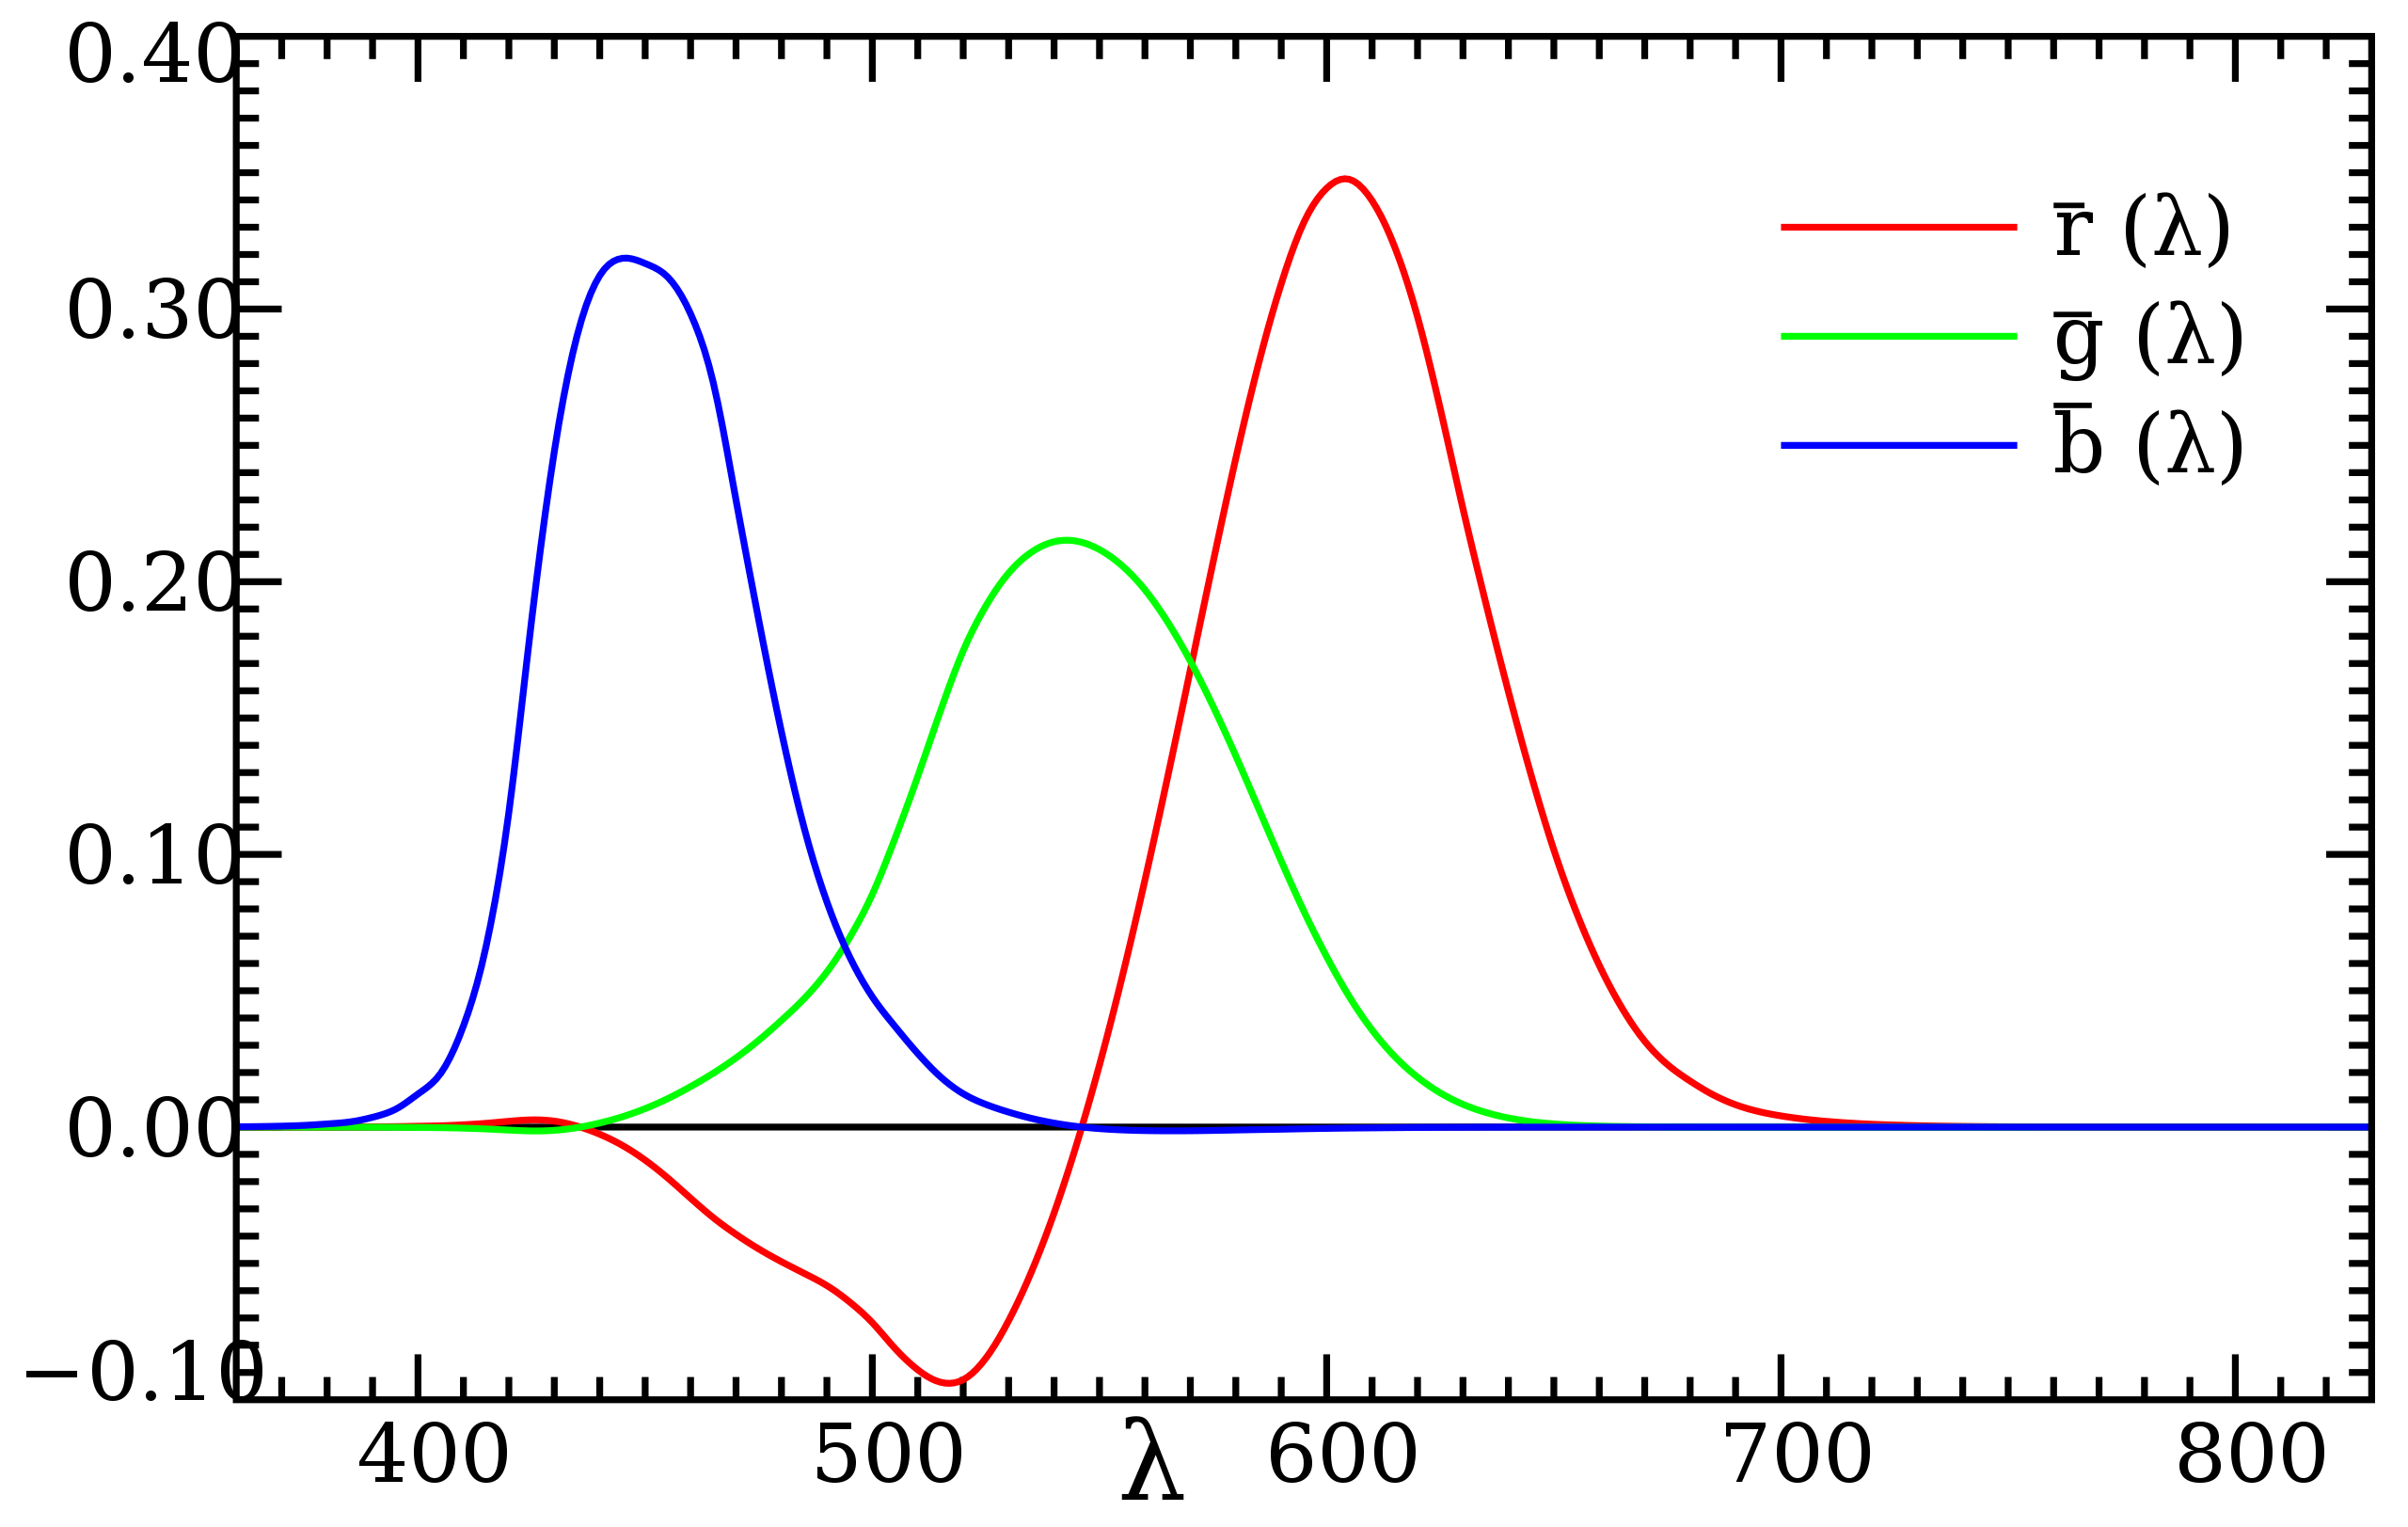
\includegraphics[width=.7\linewidth]{figures/CIE1931_RGBCMF.svg.png}
\end{bonus}

\begin{bonus}[Farbmodell]{CIE 1931-XYZ}
    % TODO: https://de.wikipedia.org/wiki/CIE-Normvalenzsystem#Der_CIE-Normalbeobachter_von_1931_und_1964
    Da negative Werte aus praktischen Gründen (z. B. Rechenschiebern) unerwünscht sind, werden die $\overline{r}$,$\overline{g}$, $\overline{b}$-Farbabgleichsfunktionen linear transformiert.
    Es ergeben sich daraus die $\overline{x}$,$\overline{y}$, $\overline{z}$-\emph{Spektralwertfunktionen}, die den Normalbeobachter charakterisieren.

    Mit Hilfe dieser $\overline{x}$,$\overline{y}$, $\overline{z}$-Spektralwertfunktionen lässt sich die Farbwahrnehmung eines durchschnittlichen Menschen (Normalbeobachter) aus einem gemessenen Lichtspektrum berechnen.
    Dazu werden die Spektralwertfunktionen skalar mit dem gemessenen Lichtspektrum multipliziert.
    Das Ergebnis sind 3 Zahlenwerte:
    (X,Y,Z), wobei Y ein Maß für die Helligkeit liefert.

    Mathematisch gesehen handelt es sich bei der Transformation um eine lineare Koordinatentransformation:
    Aus 3 Werten der $\overline{r}$,$\overline{g}$, $\overline{b}$-Farbabgleichsfunktionen  (R,G,B) die zu der Wellenlänge $\lambda$ gehören, werden mit Hilfe einer Transformationsmatrix die entsprechenden 3 Zahlenwerte (X,Y,Z) der Spektralwertfunktionen im XYZ-Farbraum bestimmt.

    Die Zahlenwerte der Transformationsmatrix sind für diesen Zweck fest vorgegeben:
    \[
        \begin{bmatrix}
            X \\ Y \\ Z
        \end{bmatrix}
        =
        \begin{bmatrix}
            2,768892 & 1,751748 & 1,130160 \\
            1        & 4,590700 & 0,060100 \\
            0        & 0,056508 & 5,594292
        \end{bmatrix}
        \cdot
        \begin{bmatrix}
            R \\ G \\ B
        \end{bmatrix}
    \]

    \centering
    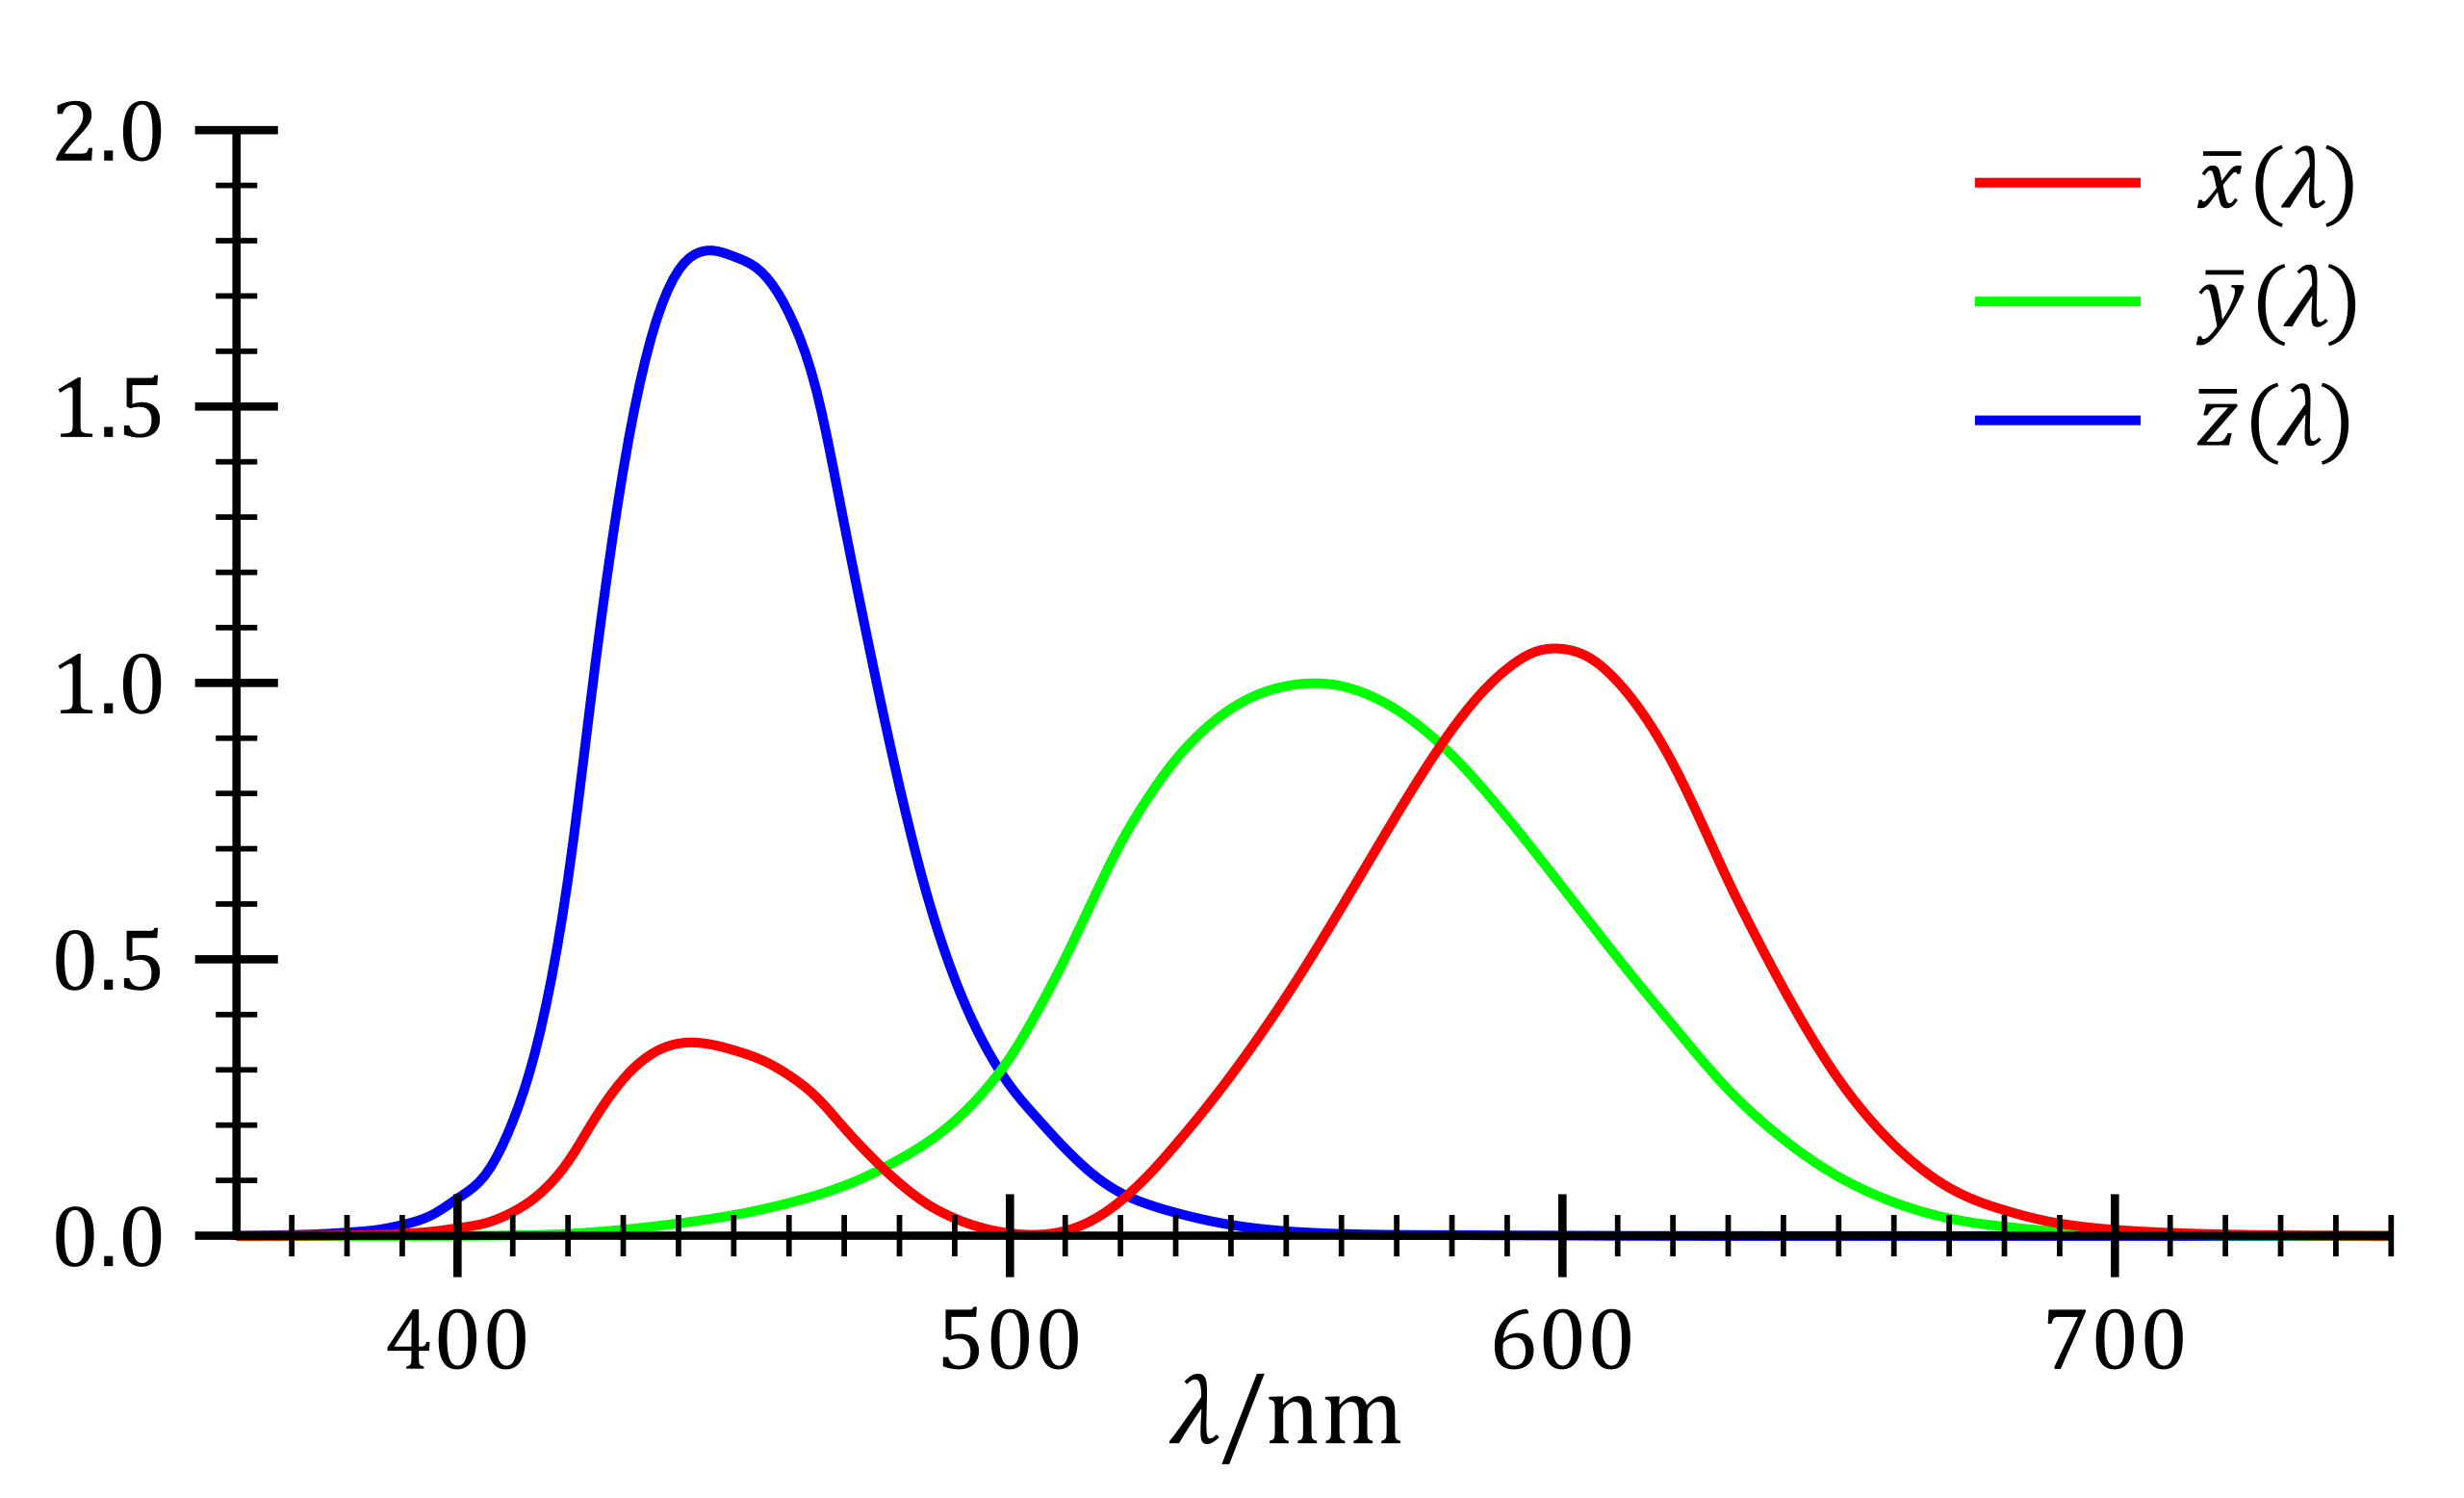
\includegraphics[width=.7\linewidth]{figures/CIE_1931_XYZ_Color_Matching_Functions.png}
\end{bonus}

\begin{bonus}[Farbmodell]{CIE xyY}
    % TODO: https://de.wikipedia.org/wiki/CIE-Normvalenzsystem#Der_CIE-Normalbeobachter_von_1931_und_1964
    Man kann Farbe in Helligkeit und Farbart (Farbton + Farbsättigung) separieren.

    In CIE XYZ ist Y als Helligkeit definiert.
    Umrechnung in \emph{CIE xyY}:
    \[
        x = \frac{X}{X + Y + Z} \quad
        y = \frac{Y}{X + Y + Z} \quad
        z = \frac{Z}{X + Y + Z} = 1 - (x + y)
    \]
    \[
        x + y + z = 1
    \]

    TODO
\end{bonus}

\begin{defi}[Farbmodell]{RGB}
    Ein \emph{RGB-Farbraum} ist ein additiver Farbraum, der Farbwahrnehmungen durch das additive Mischen dreier Grundfarben (Rot, Grün und Blau) nachbildet.
    Das Farbsehen des Menschen ist von drei Zapfentypen geprägt.
    Dieser Farbraum basiert im Prinzip auf der Dreifarbentheorie.

    Der RGB-Farbraum lässt sich als linearer Raum, anschaulich als Farbwürfel, darstellen.

    Die Wertebereiche für die Farbreize (R, G, B) können unterschiedlich festgelegt sein.
    Die klassische Darstellung lässt Werte zwischen 0 und 1 (d. h. 0 Prozent und 100 Prozent) zu;
    dies orientiert sich an der praktischen klassischen Realisierung mittels Dämpfung vorhandenen Lichts.
    Computerorientierte Anwendungen verwenden häufig die an der klassischen Form der Abspeicherung angelehnte Schreibweise, es werden Ganzzahlen zwischen 0 und einer Maximalzahl wie 255 abgespeichert.

    Da die Intensitätswahrnehmung des Menschen nichtlinear ist, wird meist eine nichtlineare Kodierung für die Luminanz vorgenommen. Diese wird häufig als Gamma-Korrektur bezeichnet, da die ersten Implementierungen die Potenzfunktion $Y \sim L^{\frac{1}{\gamma}}$ als Ansatz nutzten.
    Der Koeffizient Gamma mit $\gamma > 1$  beschreibt die Krümmung der Kurve.
    Die inverse Funktion ist $L \sim Y^\gamma$.

    Vorteile:
    \begin{itemize}
        \item RGB ist gut geeignet zum Programmieren von Hardware
    \end{itemize}

    Nachteile:
    \begin{itemize}
        \item Distanz zwischen zwei Punkten entspricht nicht der menschlichen Farbwahrnehmung
        \item Helligkeitsänderungen nicht-linear
        \item Jede Bewegung im Koordinatensystem führt zu einer Änderung von Farbton, Sättigung und Helligkeit (Farbauswahl schwierig und nicht intuitiv)
    \end{itemize}

    \centering
    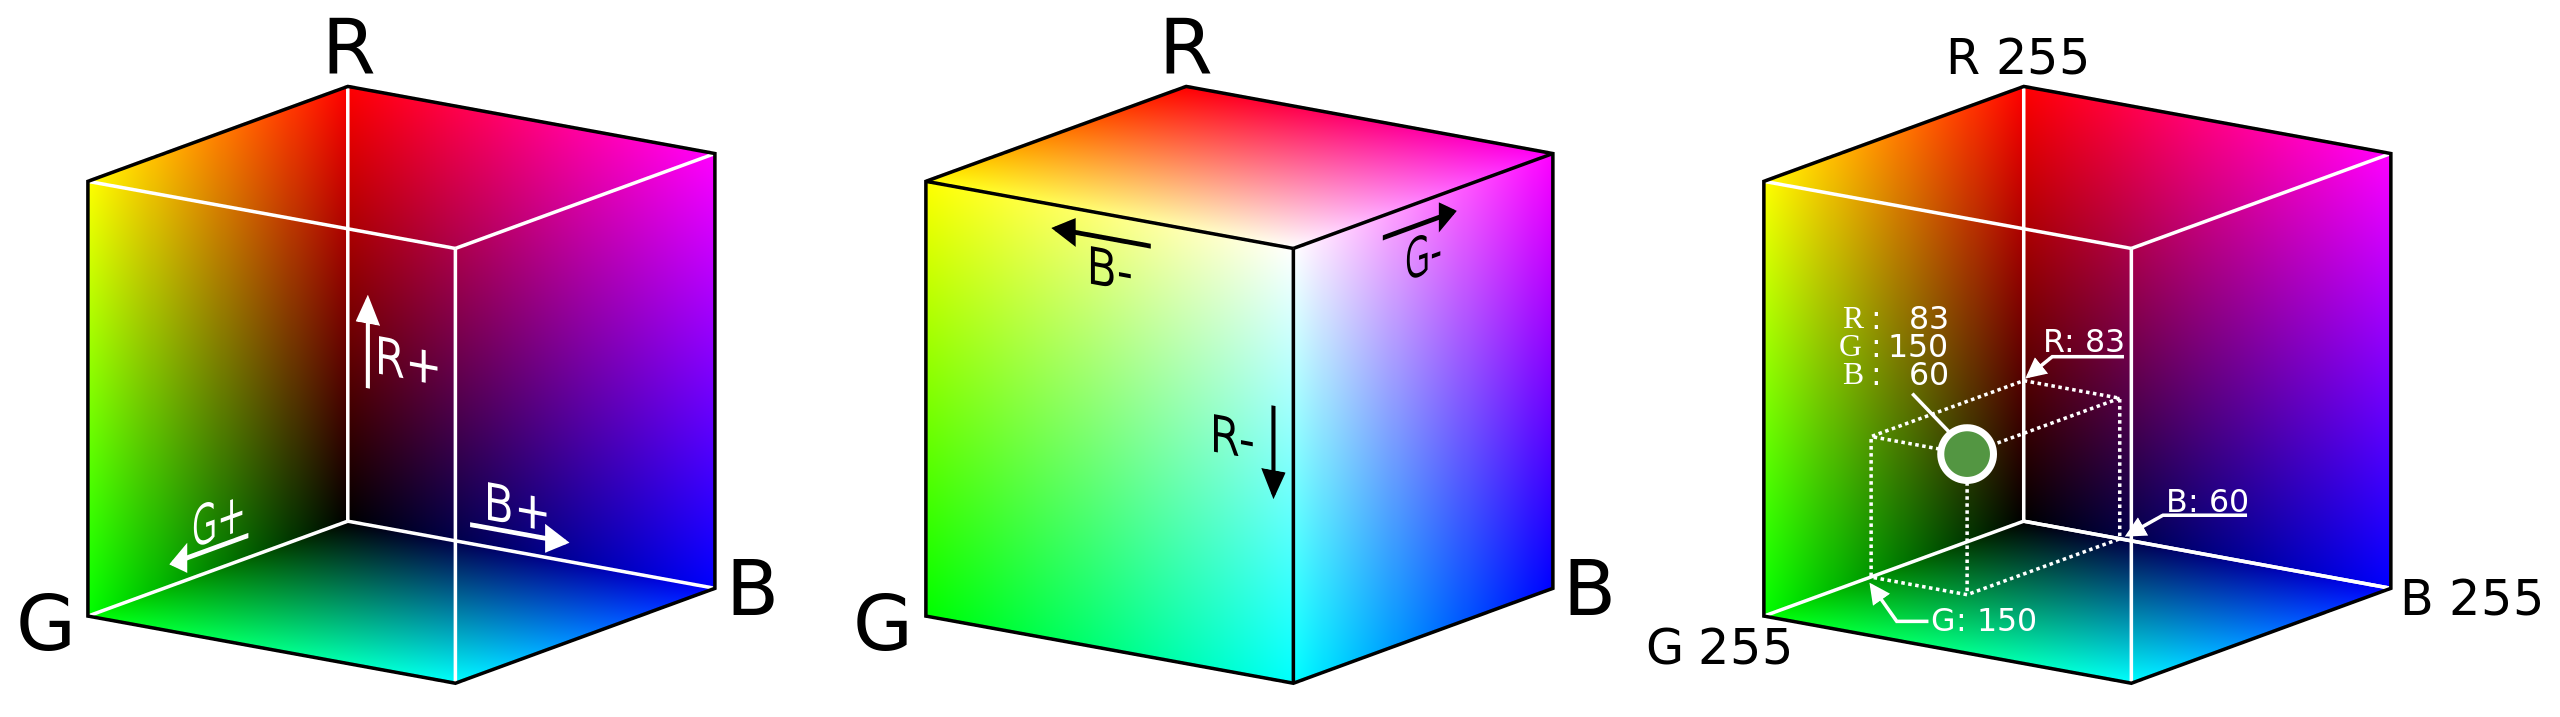
\includegraphics[width=.7\linewidth]{figures/RGB_color_cube.png}
\end{defi}

\begin{defi}{Entsättigung}
    \emph{Entsättigung} ist die gleichmäßige Reduzierung von Farbe.
\end{defi}

\begin{defi}[Farbmodell]{CMYK}
    Das \emph{CMYK-Farbmodell} ist ein subtraktives Farbmodell, das die technische Grundlage für den modernen Vierfarbdruck bildet.
    Die englischsprachige Abkürzung CMYK, die auch in vielen nicht-englischsprachigen Ländern verwendet wird, steht für die drei Farbbestandteile Cyan, Magenta, Yellow und den Schwarzanteil, der traditionell als Key bezeichnet wird.

    Das CMYK-Farbmodell ist ein geräteabhängiges Farbmodell.
    Es beschreibt vordergründig nur, zu welchen Anteilen ein Ausgabegerät die Farbbestandteile kombinieren soll, um einen bestimmten Farbton herzustellen. Wie ein solcher Farbton im Druck aussieht, hängt von der Drucktechnik, den eingesetzten Grundfarben und sogar von der zu bedruckenden Oberfläche ab.

    Die Umrechnung vom RGB-Farbraum zum CMY-Farbraum erfolgt wie folgt:
    \[
        \begin{pmatrix}
            C \\ M \\ Y
        \end{pmatrix}
        =
        \begin{pmatrix}
            1 - R \\
            1 - G \\
            1 - B
        \end{pmatrix}
    \]

    Die zusätzliche Druckfarbe Schwarz (Key), für die das CMYK-Farbmodell entworfen wurde, ist für den Zusammendruck der drei Bunttöne nötig, da diese theoretisch, aber nicht praktisch ein ausreichend tiefes Schwarz ergeben.
    Um CMY in CMYK umzurechnen gibt es verschiedene Varianten, z. B.:
    \begin{itemize}
        \item lineare Reduktion der Farben mit wachsendem $K$:
              \[
                  \begin{pmatrix}
                      C' \\ M' \\ Y' \\ K'
                  \end{pmatrix}
                  =
                  \begin{pmatrix}
                      C - K \\
                      M - K \\
                      Y - K \\
                      K
                  \end{pmatrix}
              \]
        \item stärkere Farben in dunklen Bereichen:
              \[
                  \begin{pmatrix}
                      C' \\ M' \\ Y' \\ K'
                  \end{pmatrix}
                  =
                  \begin{pmatrix}
                      (C - K) \cdot s \\
                      (M - K) \cdot s \\
                      (Y - K) \cdot s \\
                      K
                  \end{pmatrix}
                  , \quad s \begin{cases}
                      \frac{1}{1 - K} & K < 1        \\
                      1               & \text{sonst}
                  \end{cases}
              \]
    \end{itemize}
\end{defi}

\begin{defi}[Farbmodell]{HSV}
    % TODO: https://de.wikipedia.org/wiki/HSV-Farbraum
    Der \emph{HSV-Farbraum} ist der Farbraum etlicher Farbmodelle.
    Hier ist der Farbort einer Farbe definiert mit Hilfe der drei Koordinaten:
    \begin{itemize}
        \item Farbwert (englisch hue): Farbwinkel auf dem Farbkreis (0° für Rot, 120° für Grün, 240° für Blau)
        \item Farbsättigung (saturation): (0 \% = Neutralgrau, 50 \% = wenig gesättigte Farbe, 100 \% = gesättigte, reine Farbe)
        \item Hellwert (value; auch Dunkelstufe genannt): (0 \% = keine Helligkeit, 100 \% = volle Helligkeit)
    \end{itemize}

    In Fragen der Farbnachstellung wird das HSV-Modell gegenüber den Alternativen RGB und CMYK bevorzugt, weil es der menschlichen Farbwahrnehmung stärker entspricht (beispielsweise ist es im RGB-Modell schwer, sich Gelb als Mischung von Rot und Grün vorzustellen).
    Für die Farbmischung kann man unmittelbar den gewünschten Farbton wählen und dann entscheiden, wie gesättigt und wie hell (oder dunkel) dieser sein soll, oder ob eine andere Farbnuance passender ist:

    Der Farbwinkel spezifiziert die dominante Wellenlänge der Farbe, mit Ausnahme des Bereiches zwischen Blauviolett und Rot (240° und 360°), wo er eine Position auf der Purpurlinie angibt.

    Die Sättigung entspricht der Zumischung von purem Weiß (d. h. Licht mit gleichen Intensitäten in allen Wellenlängen) zu einer simulierten Spektralfarbe (oder vielmehr der entsprechenden Spaltbreite um die dominante Wellenlänge herum);
    dabei entspricht stärkere Weiß-Zumischung einer geringeren Sättigung.

    Die Helligkeit ist ein Parameter für den Gesamtenergieinhalt bzw. für die maximale Amplitude des Lichts;
    die Dunkelstufe ergänzt diesen Wert im Gegensätzlichen.
    Nachteilig bei der Dunkelstufe ist, dass Weiß und ein beliebiger Farbton die gleiche Sättigung haben können.

    In diesem System wird Weiß als Buntfarbe behandelt.
    In der Praxis wiederum ist die Umwandlung eines Farbbildes in ein Schwarz-Weiß-Bild durch Ändern nur einer Koordinate nicht möglich.

    \centering
    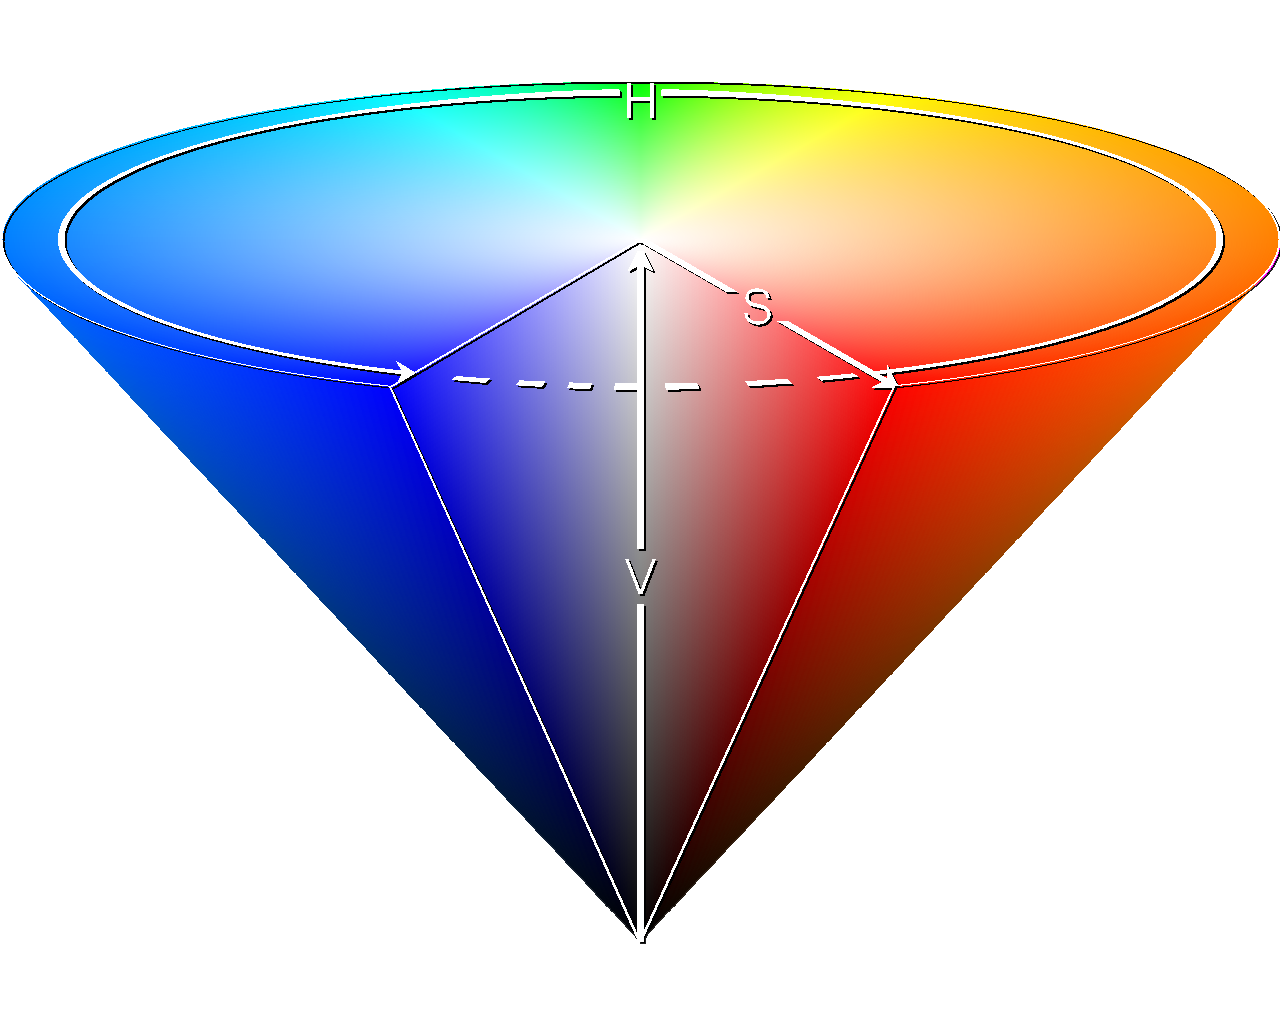
\includegraphics[width=.4\linewidth]{figures/HSV_cone.png}
\end{defi}

\begin{defi}[Farbmodell]{HSI}
    An den Bedürfnissen der Farbmetrik und der phototechnischen Reproduktion orientiert sich das \emph{HSI-Modell}.
    Auch hierbei steht H für Buntwert (hue) und S für Sättigung.

    Der Unterschied bezieht sich auf die dritte Koordinate, die Lichtintensität I.

    TODO: Umrechnung
\end{defi}

\begin{bonus}[Farbmodell]{HSL}
    Der \emph{HSL-Farbraum} hat die Parameter Farbwinkel $H$, Farbsättigung $S$ und Farbhelligkeit $L$.

    Im Gegensatz zum HSV-Farbraum wird er jedoch auf den zwischen Weiß und Schwarz liegenden Graupunkt als neutrales Grau bezogen.
    Der Graupunkt liegt in der Mitte und die Buntwerte außen, der Farbkörper wird daher als Doppelkegel, (Doppel-)Zylinder oder sechsseitiges Prisma dargestellt.

    \centering
    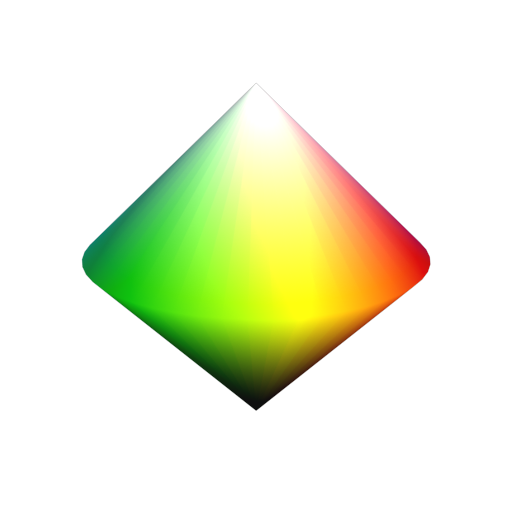
\includegraphics[width=.4\linewidth]{figures/HSL_cone.png}
\end{bonus}

\begin{defi}[Farbmodell]{YUV}
    % TODO: https://de.wikipedia.org/wiki/YUV-Farbmodell 
    Das \emph{YUV-Farbmodell} wird beim analogen Farbfernsehen nach den Normen PAL und NTSC verwendet.

    Es verwendet zur Darstellung der Farbinformation zwei Komponenten:
    \begin{itemize}
        \item die Luminanz (luma, Lichtstärke pro Fläche, d. h. Leuchtdichte) $Y$ und
        \item die Chrominanz (Farbanteil, chroma), wobei diese aus den zwei Unterkomponenten $U$ und $V$ besteht.
    \end{itemize}

    Wie das Farbdreieck, von dem es abgeleitet wurde, geht das YUV-Farbmodell von einem Modell mit linearer Addition der Farbreize aus.
    Diese Modelle sind mit Hilfe einer Matrix ineinander überführbar.

    Zur Berechnung des Luma-Signals $Y$ werden die zugrundeliegenden RGB-Daten zunächst mit dem Gamma-Wert des Ausgabegerätes verrechnet;
    man erhält ein $R'G'B'$-Signal.
    Die drei Einzelkomponenten werden mit unterschiedlicher Gewichtung addiert, um die Helligkeitsinformation zu bilden.

    Die Gewichtung der Komponenten ist erforderlich, da einige Aspekte des Farbensehens des menschlichen Auges berücksichtigt werden müssen.
    So wird beispielsweise Grün heller wahrgenommen als Rot, dieses wiederum heller als Blau.
    Diese unterschiedliche Gewichtung wird in folgender (per Definition exakten) Umrechnungsformel berücksichtigt:
    \[
        Y := 0.299 \cdot R + 0.587 \cdot G + 0.114 \cdot B
    \]

    Die \emph{Chrominanzsignale} (auch Farbdifferenzsignale) $U$ und $V$ enthalten die Farbinformation. Sie entstehen aus der Differenz zwischen Blauanteil B und Luminanz Y bzw. zwischen Rotanteil und Luminanz sowie einer weiteren Reduktion;
    auch diese Formeln sind per Definition exakt:
    \[
        U := 0.493 \cdot (B - Y)
    \]
    \[
        V := 0.877 \cdot (R - Y)
    \]

    Aus den drei erzeugten Komponenten $Y$, $U$ und $V$ können später wieder die einzelnen Farbanteile der Grundfarben berechnet werden durch die jeweiligen Rücktransformationen.

    \centering
    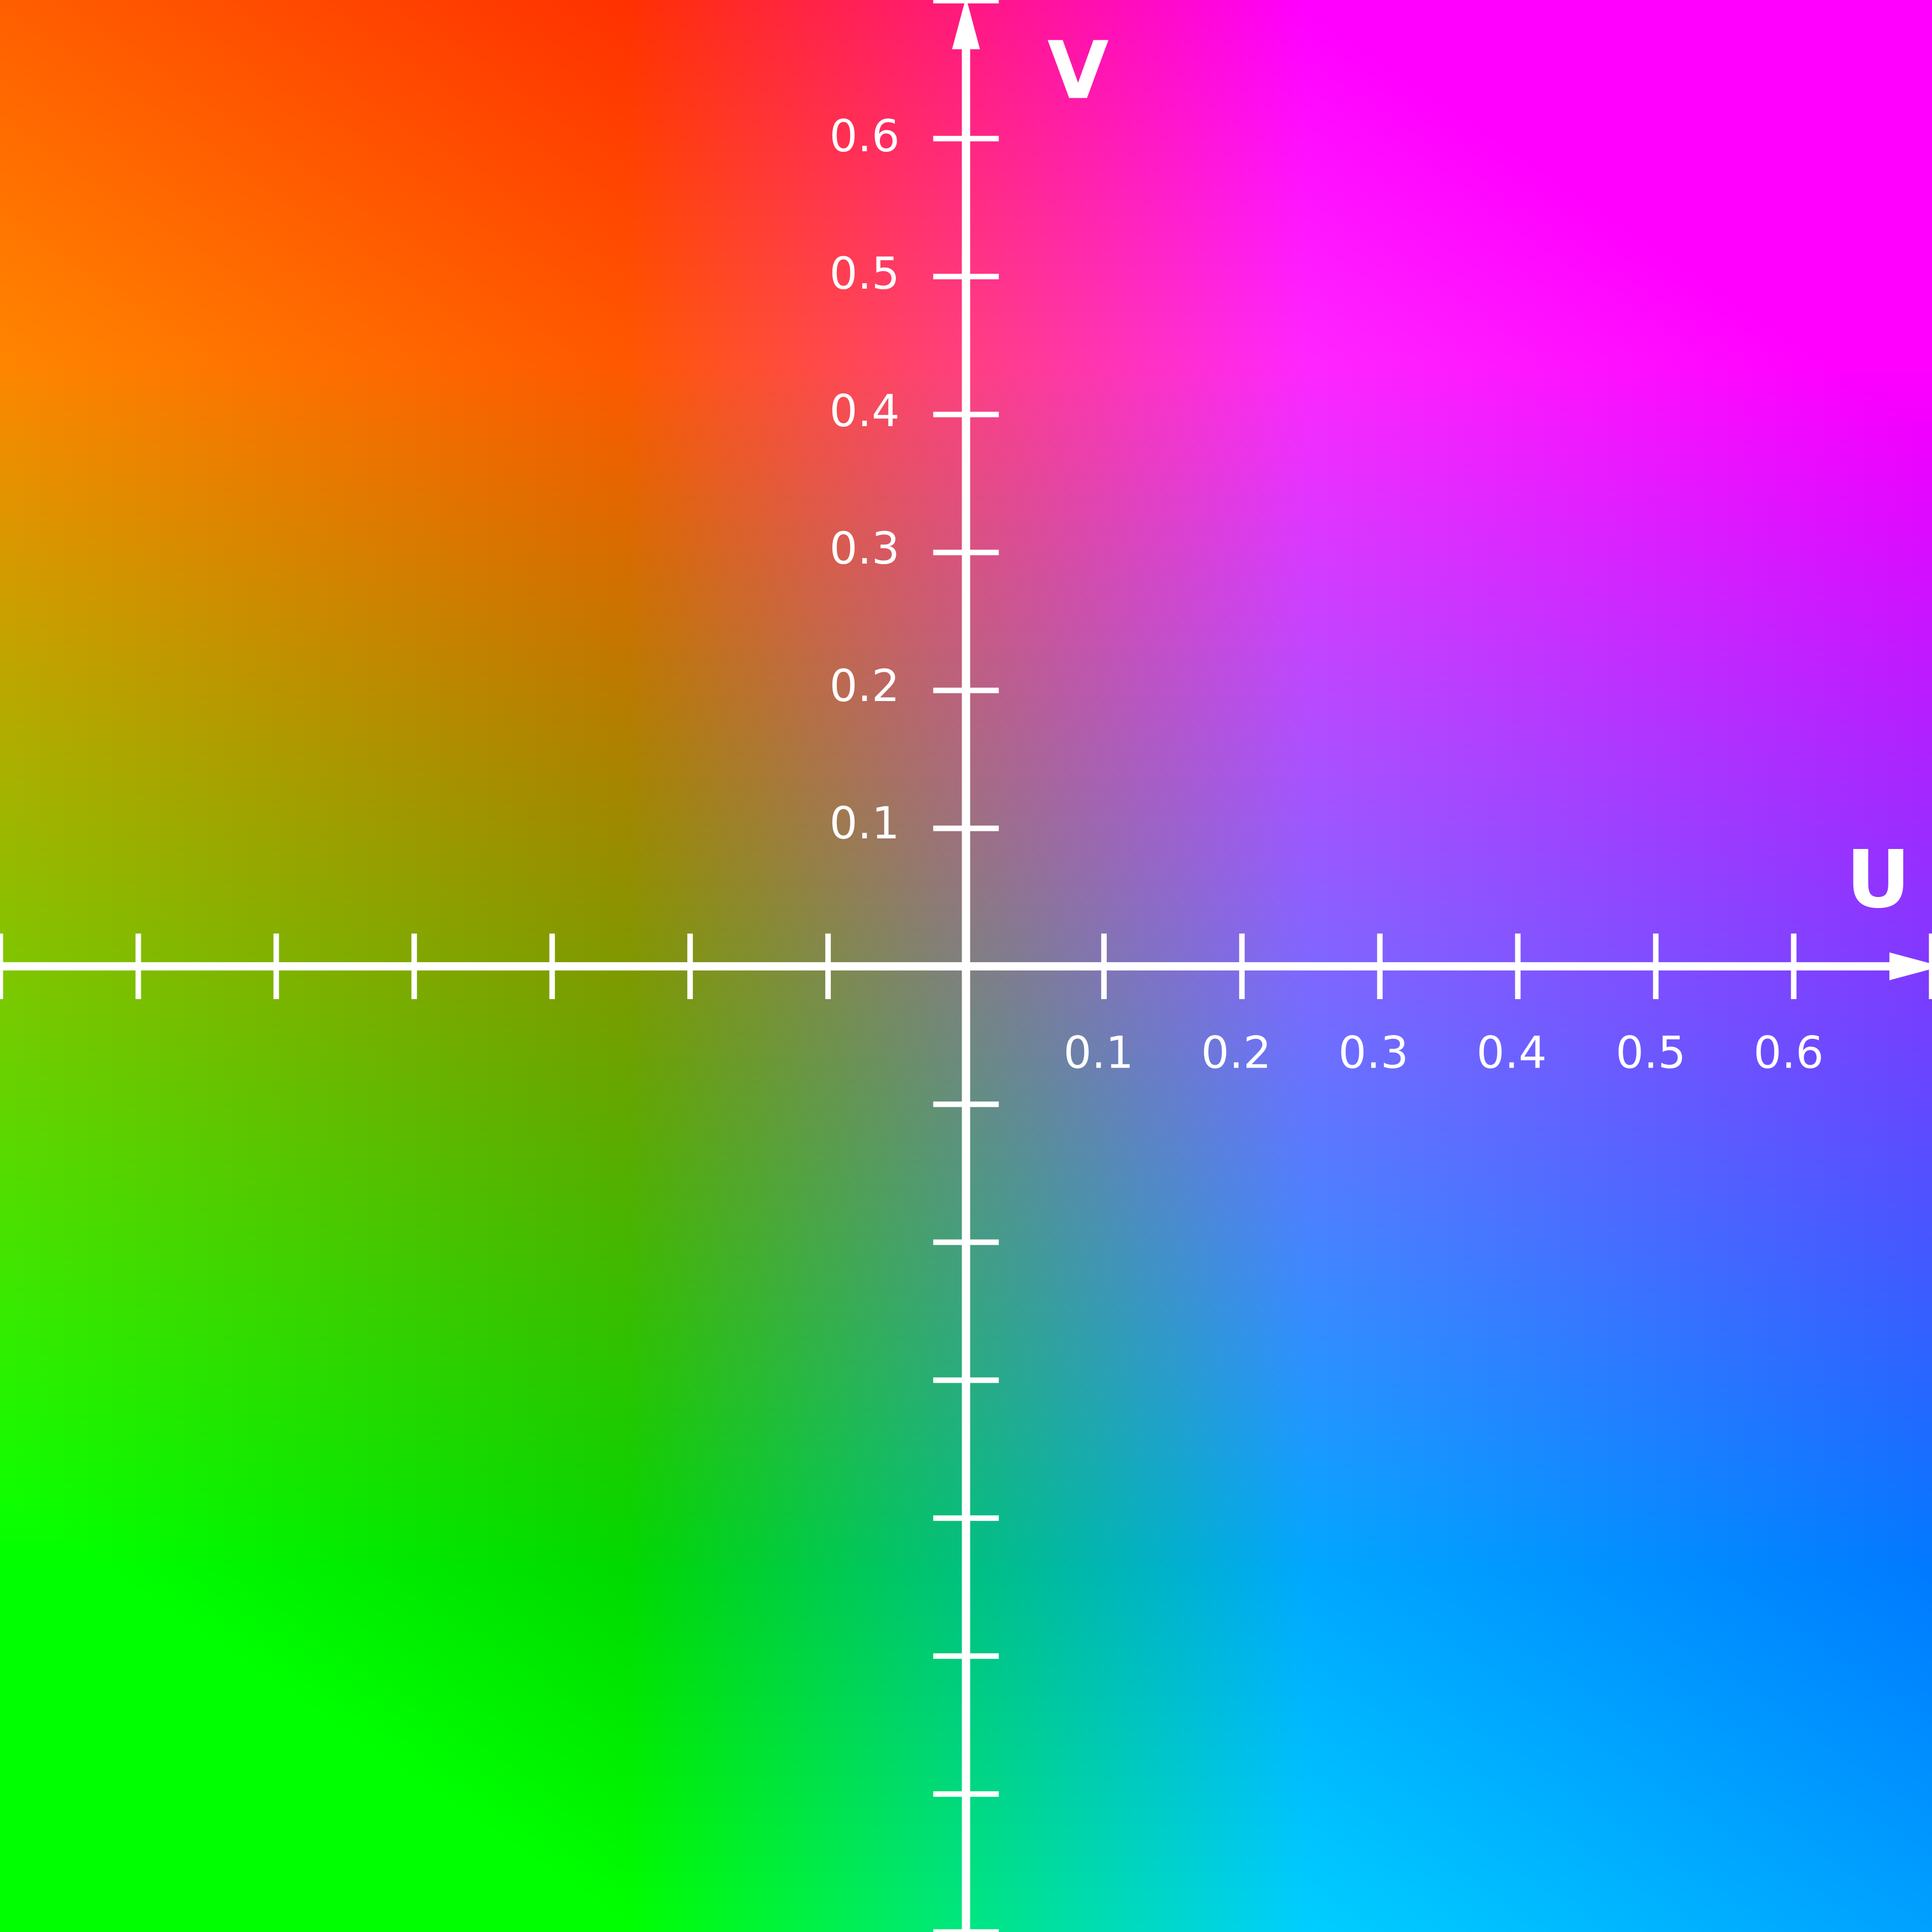
\includegraphics[width=.4\linewidth]{figures/YUV-UV_Scaled_Y0.5_70_percent.png}

    UV-Fläche des YUV-Farbmodells im RGB-Farbraum auf einer Helligkeitsebene von $Y = 0.5$.
\end{defi}

\begin{defi}[Farbmodell]{YCbCr}
    % TODO: https://de.wikipedia.org/wiki/YCbCr-Farbmodell
    Das \emph{YCbCr-Farbmodell} wurde für das Digitalfernsehen nach der Norm PAL entwickelt, wird heute aber auch beim digitalen NTSC-Fernsehen genutzt.

    Das YCbCr-Modell teilt die Farbinformation in die Grundhelligkeit $Y$ und die zwei Farbkomponenten $Cb$ (Blue-Yellow Chrominance) und $Cr$ (Red-Green Chrominance) auf.
    Mit $Y$ wird hier die Helligkeitsachse aus dem CIE-Normvalenzsystem verwendet.
    Sie entspricht der Hellempfindlichkeit des Auges, die im grünen Spektralbereich am größten ist.
    Chrominance oder kurz Chroma bedeutet Buntheit im Allgemeinen und Farbigkeit in Bezug auf Helligkeit-Farbigkeits-Modelle.

    Vergleicht man die beiden Separationen des Bildbeispiels in YUV und YCbCr, wird ersichtlich, dass der Helligkeitskanal ein völlig unbuntes Graustufenbild zeigt und, dass lediglich die Chrominanzachsen U und V in der Farbtafel andere Farbtöne durchschneiden als Cb und Cr.
    Cb ist also ein Maß für die Abweichung der Farbigkeit von Grau in Richtung Blau/Gelb, Cr ist die entsprechende Maßzahl in Richtung Rot/Türkis.

    \centering
    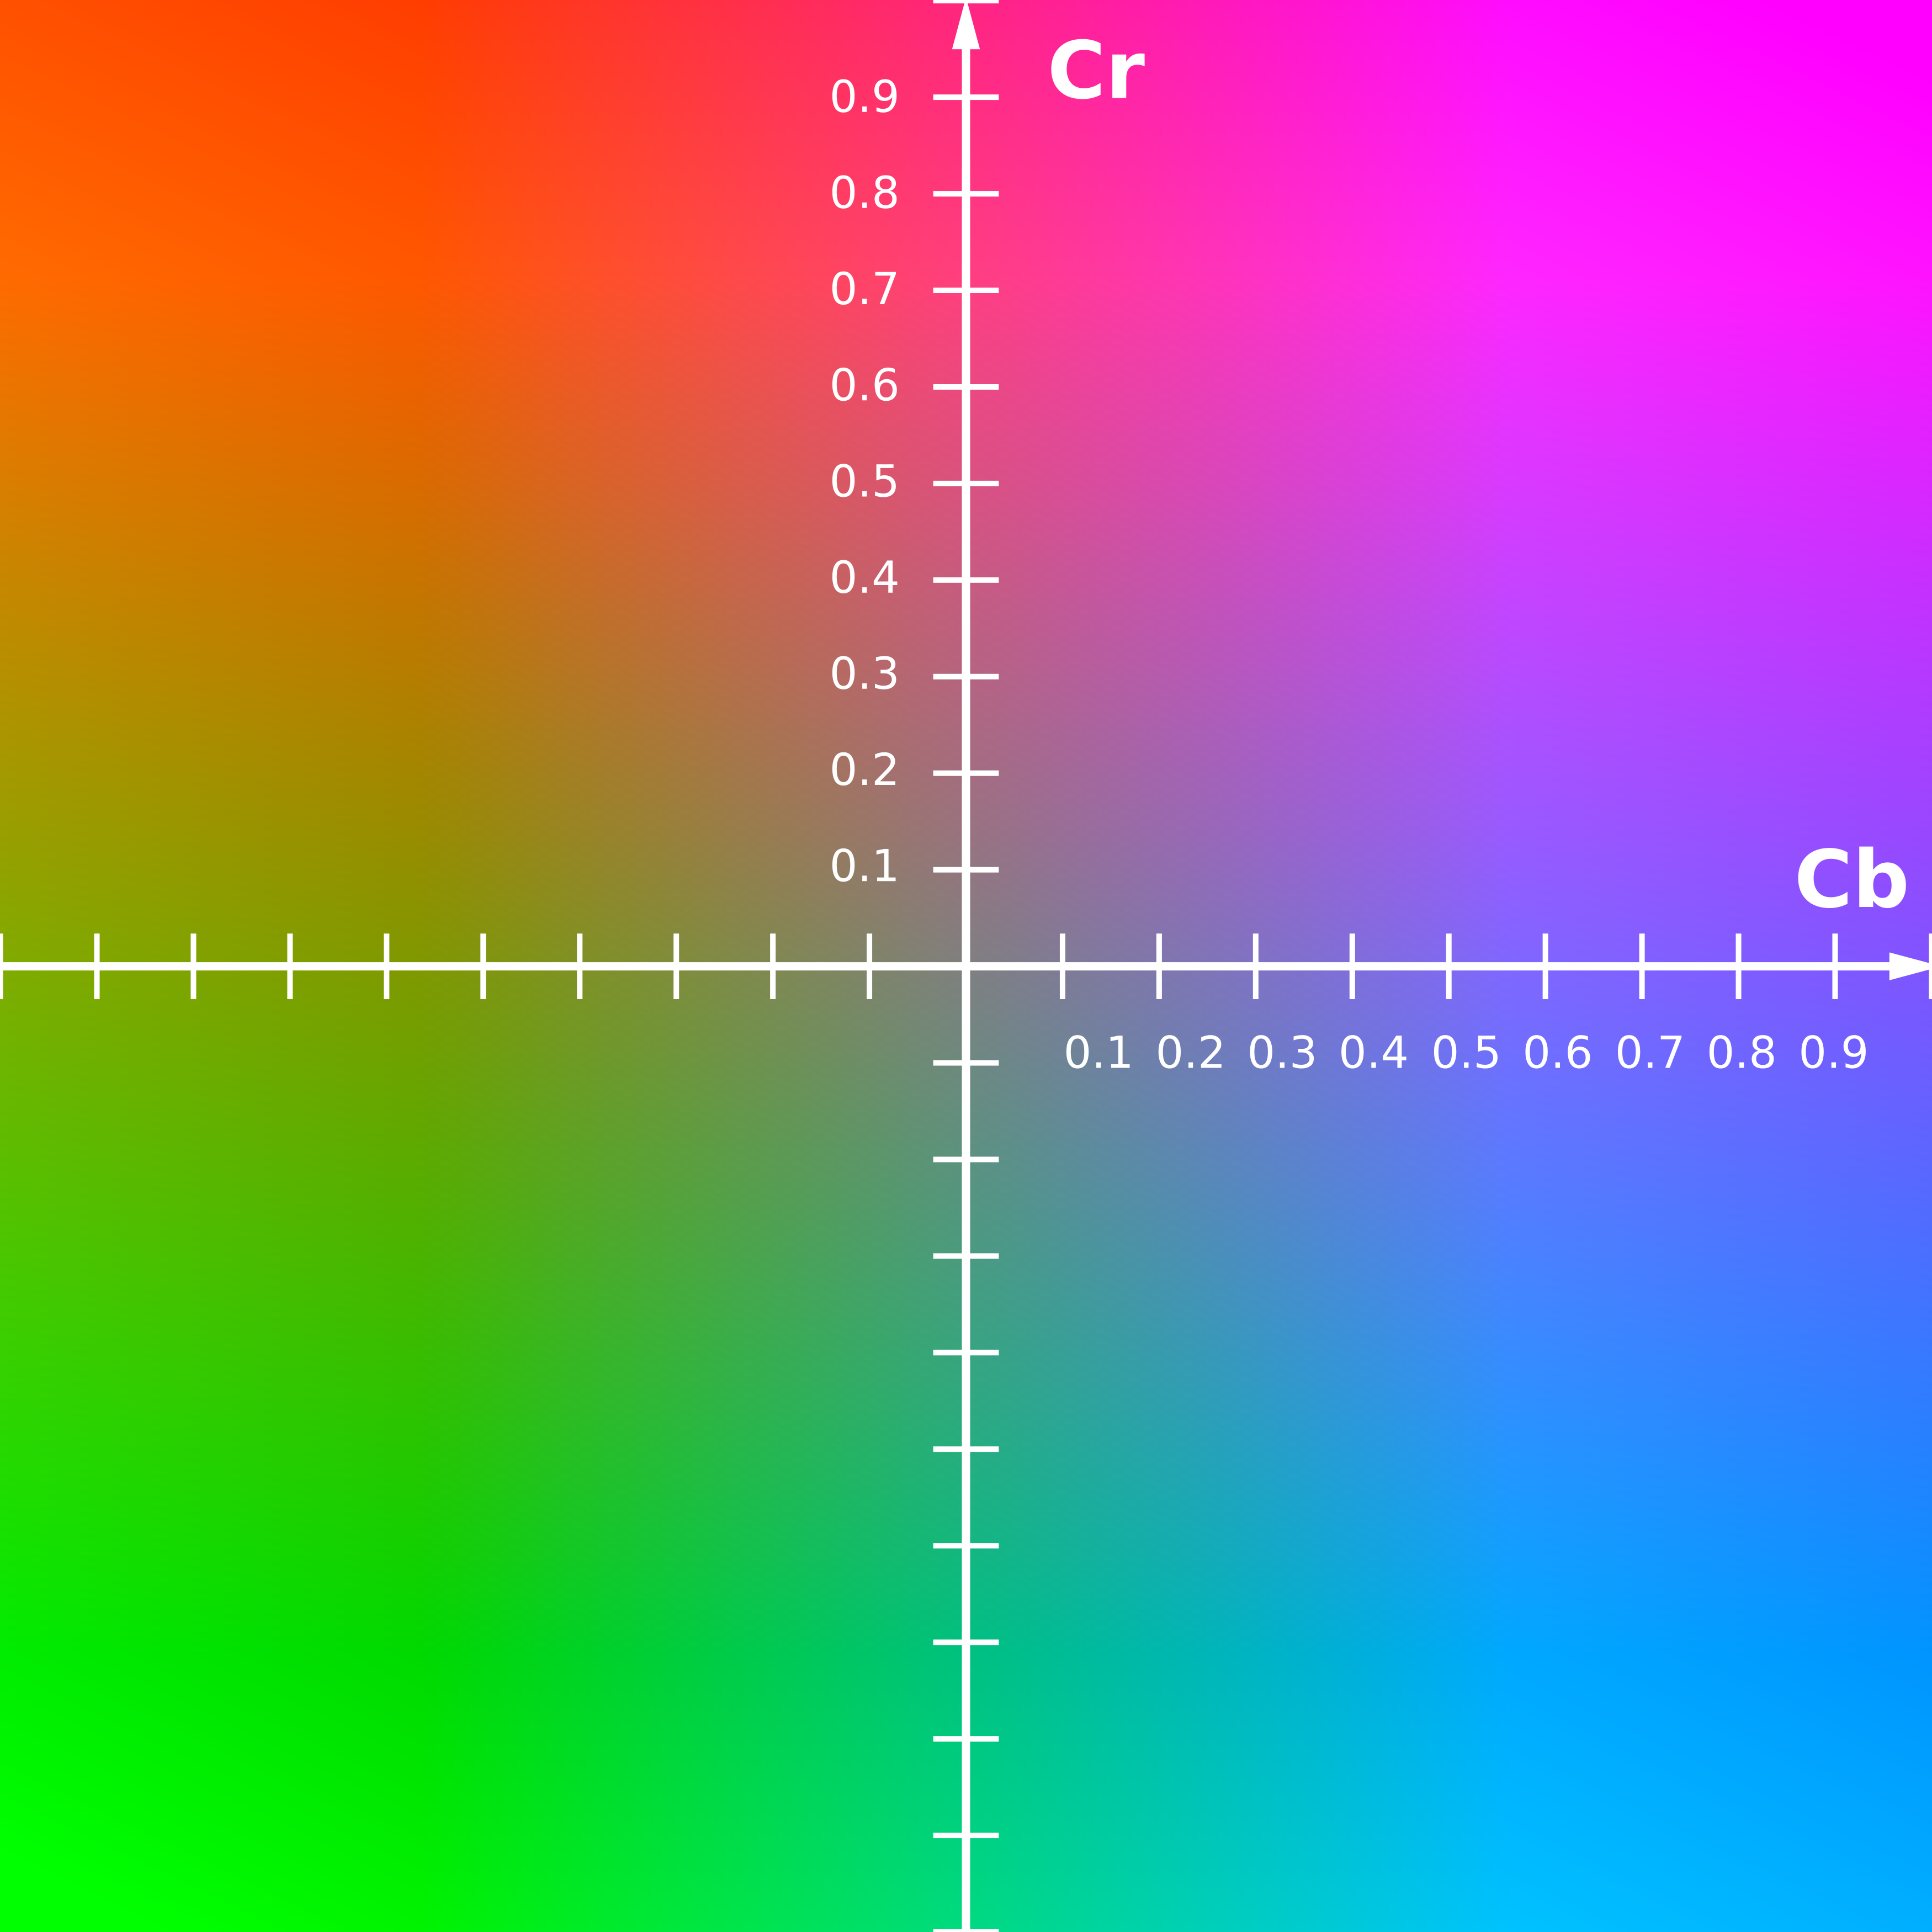
\includegraphics[width=.4\linewidth]{figures/YCbCr-CbCr_Scaled_Y50.png}

    CbCr-Fläche des YCbCr-Farbmodells im RGB-Farbraum auf einer Helligkeitsebene von $Y = 0.5$.
\end{defi}

\begin{bonus}[Farbmodell]{CIE L*a*b*}
    TODO
\end{bonus}

\begin{bonus}[Farbmodell]{CIE LCh}
    TODO
\end{bonus}